\documentclass[12pt,a4paper]{amsart}
\usepackage[slovene]{babel}
%\usepackage[cp1250]{inputenc}
\usepackage[T1]{fontenc}
\usepackage[utf8]{inputenc}
\usepackage{amsmath,amssymb,amsfonts}
\usepackage{url}
\usepackage[normalem]{ulem}
\usepackage[dvipsnames,usenames]{color}
\usepackage{graphicx}

% Oblika strani
\textwidth 15cm
\textheight 24cm
\oddsidemargin.5cm
\evensidemargin.5cm
\topmargin-5mm
\addtolength{\footskip}{10pt}
\pagestyle{plain}
\overfullrule=15pt % oznaci predlogo vrstico

% Ukazi za matematična okolja
\theoremstyle{definition} % tekst napisan pokončno
\newtheorem{definicija}{Definicija}[section]
\newtheorem{primer}[definicija]{Primer}
\newtheorem{opomba}[definicija]{Opomba}

\renewcommand\endprimer{\hfill$\diamondsuit$}


\theoremstyle{plain} % tekst napisan poševno
\newtheorem{lema}[definicija]{Lema}
\newtheorem{izrek}[definicija]{Izrek}
\newtheorem{trditev}[definicija]{Trditev}
\newtheorem{posledica}[definicija]{Posledica}

\begin{document}
%%%%%%%%%%%%%%%%%%%%%%%%%%%%%%%%%%%%%%%%%%%%%%%%%%%%%%%%%%%%%%%%%%%%%%%%%%%%%%%%%%%%%%%%%%%%%%%%%%%%%%%%%%%%%%%%%%%%%%%%%%%%%%%%%%%%%%%%%%%%%%
\title{Izogibanje napakam verjetnostnega sklepanja v pravni praksi z uporabo Bayesovih mrež}
\author{Neža Kržan}
\maketitle

%%%%%%%%%%%%%%%%%%%%%%%%%%%%%%%%%%%%%%%%%%%%%%%%%%%%%%%%%%%%%%%%%%%%%%%%%%%%%%%%%%%%%%%%%%%%%%%%%%%%%%%%%%%%%%%%%%%%%%%%%%%%%%%%%%%%%%%%%%%%%%
%%%%%%%%%%%%%%%%%%%%%%%%%%%%%%%%%%%%%%%%%%%%%%%%%%%%%%%%%%%%%%%%%%%%%%%%%%%%%%%%%%%%%%%%%%%%%%%%%%%%%%%%%%%%%%%%%%%%%%%%%%%%%%%%%%%%%%%%%%%%%%
\section{Zmote v kazenskem pravu}
Ker večina ljudi pri razmišljanju o verjetnosti dela osnovne napake, obstaja mnogo zmot, ki izhajajo iz osnovnega razumevanja pravil
teorije verjetnosti. Številne od teh zmot so zlasti posledica napačnega razumevanja pogojne verjetnosti. Bolj znana primera takih zmot sta
Tožilčeva zmota(angl. Prosecutor’s fallacy) in Zmota obrambnega odvetnika(angl. Defense attorney's fallacy). Čeprav so posledice tožilčeve zmote 
lahko hujše kot posledice zmote obrambnega odvetnika, so porote morda bolj dovzetne za slednjo kot za prvo. \\\\
Če upoštevamo vzročno verigo dokazov, predstavljeno na sliki 1, lahko razvrstitev zmot posplošimo na večino vrst dokazov. Ta shema 
nam omogoča klasifikacijo napak v sklepanju.
\begin{figure}[!ht]\label{fig:slika_3}
    \centering
    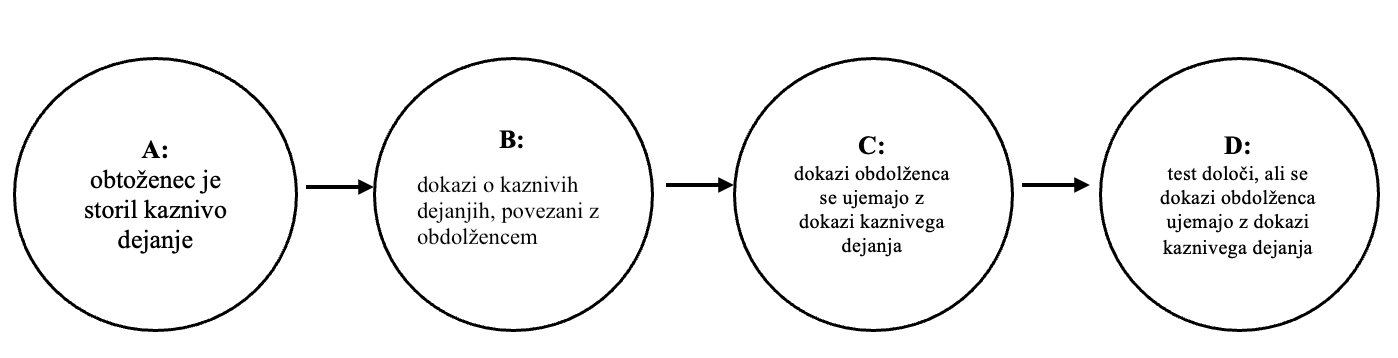
\includegraphics[scale=0.60]{slika_3.png}
    \caption{Vzorčna veriga dokazov}
\end{figure}
\\
Ta analiza je močno odvisna od pojma "pogostost ujemajočih se lastnosti", označenega kot $F$(lastnosti). Ta se včasih imenuje 
tudi "verjetnost naključnega ujemanja". V našem vzročno-posledičnem okviru je $F$(lastnosti) enakovreden bolj formalno opredeljeni verjetnosti 
$P(C \lvert \neg B)$, t.j. verjetnost, da oseba, ki ni vpletena v kaznivo dejanje, po naključju zagotovi dokaze, ki se ujemajo.\\\\
S tem vzročno-posledičnim okvirom lahko opišemo vrsto različnih pogostih zmot, ki so posledica napačnega razumevanja pogojne verjetnosti:\\
\textit{Napaka glavne težave}: pri tem enačimo $P(C \lvert \neg B)$ s $P(\neg A \lvert C)$. To je bilo 
imenovano tožilska zmota - presega napako predhodne verjetnosti, saj si jo lahko predstavljamo kot dopolnitev te napake z dodatno napačno 
predpostavko $P(A) = P(B)$.\\\\
\textit{Napaka verjetnosti $P(\text{drugo ujemanje})$}: gre za zmoto, ko verjetnost $P(C \lvert \neg B)$ enačimo z verjetnostjo 
(imenujmo jo $q$), da ima vsaj en nedolžen član populacije ustrezne dokaze. Posledica te napake je običajno močno pretiravanje z vrednostjo 
dokaza $C$.\\\\
\textit{Zanemarjanje predhodnih verjetnosti}: to pomeni preprosto neupoštevanje predhodnih vrednosti, kot sta $P(A)$ in $P(B)$. Na splošno 
se za zmoto zanemarjanja osnovne stopnje šteje, kadar je verjetnost dogodka podcenjena, ker dogodek ni tako nenavaden, kot se zdi, 
ali precenjena, ker je dogodek bolj nenavaden, kot se zdi.\\\\
\textit{Napaka pri številčnem preračunavanju}: pri tem gre za zamenjavo vrednosti $P(C \lvert \neg B)$ s pričakovanim številom drugih oseb, 
ki bi jih bilo treba testirati, preden bi našli ujemanje. Ta zmota prav tako pretirava z vrednostjo dokaza $C$.\\\\
\textit{Pričakovane vrednosti, ki pomenijo edinstvenost}: če je velikost populacije približno enaka $1/P(\neg B \lvert C)$, potem mora biti 
obdolženec edini primerek. Binomski izrek pokaže, da obstaja več kot 25\% verjetnost, da bosta v populaciji, katere velikost je $1/P(\neg B \lvert C)$, 
vsaj dva ujemanja.\\\\
\textit{Zmota obrambnega odvetnika}: to se zgodi, ko se dokaz $C$ šteje za nepomembnega, ker visoka predhodna verjetnost $P(\neg A)$ (kar 
se zgodi, če je na primer potencialno število osumljencev zelo veliko) še vedno povzroči visoko verjetnost $P(\neg B \lvert C)$.
\textit{Napaka baze podatkov obrambnega odvetnika}: za to napako gre, kadar verjetnost $P(\neg B \lvert C)$ temelji na drugačni populaciji, 
kot jo določa $P(B)$ ali $P(A)$.\\\\
\textit{Zasliševalčeva zmota}: v tem primeru je dokaz neposredno priznanje krivde. Če to ni potrjeno, to pomeni, da uporabljamo $P(D \lvert A)$ za 
informiranje $P(A \lvert D)$. Napaka je, da ne upoštevamo $P(D \lvert \neg A)$. Če je $P(D \lvert A) \leq P(D \lvert \neg A)$, potem dokaz 
nima vrednosti.\\\\
Poleg zmot, ki izhajajo iz osnovnega nerazumevanja pogojne verjetnosti, se druge zmote pojavijo zaradi neustreznega združevanja vpliva več dokazov:\\
\textit{Zmota odvisnih dokazov}: ta zmota, ki se včasih imenuje tudi dvojno štetje, se kaže v tem, da se dva ali več dokazov, ki so odvisni, 
obravnava, kot da bi bili neodvisni, zaradi česar je izjava o njihovi skupni verjetnosti manjša, kot bi morala biti. Poseben primer te zmote je 
\textit{logično odvisna dokazna zmota}, pri kateri en dokaz ni preprosto odvisen od drugega, ampak dejansko logično izhaja iz njega.\\\\
\textit{Napaka konjunkcije}: ta zmota se pojavi, kadar preiskovalec ne upošteva dejstva, da je dokaz sestavljen iz več kot enega negotovega dogodka, 
in mu posledično pripiše večjo verjetnost, kot bi jo moral.\\\\

%%%%%%%%%%%%%%%%%%%%%%%%%%%%%%%%%%%%%%%%%%%%%%%%%%%%%%%%%%%%%%%%%%%%%%%%%%%%%%%%%%%%%%%%%%%%%%%%%%%%%%%%%%%%%%%%%%%%%%%%%%%%%%%%%%%%%%%%%%%%%%
%%%%%%%%%%%%%%%%%%%%%%%%%%%%%%%%%%%%%%%%%%%%%%%%%%%%%%%%%%%%%%%%%%%%%%%%%%%%%%%%%%%%%%%%%%%%%%%%%%%%%%%%%%%%%%%%%%%%%%%%%%%%%%%%%%%%%%%%%%%%%%
\section{Tožilčeva zmota}
Verjetnostno utemeljevanje pravnih dokazov se torej skrči na preprost vzročni scenarij: začnemo z neko hipotezo $H$ in opazujemo nek dokaz $E$. 
Poznavanje pogojne verjetnosti $P(E \lvert H)$ nam omogoča, da spremenimo svoje prepričanje o verjetnosti $H$, če poznamo $E$. Veliko najpogostejših 
napak v sklepanju izhaja iz osnovnega nerazumevanja pogojne verjetnosti. Še posebej pogost primer je zamenjava verjetnost dokaza $E$ glede na 
hipotezo $H$ z verjetnost hipoteze $H$ glede na dokaze $E$ oziroma $P(E \lvert H)$ z $P(H \lvert E)$. To se pogosto imenuje napaka prenesenega pogojnika 
oziroma tudi tožilčeva zmota.\\\\
Tožilčeva zmota(angl. Prosecutor’s fallacy) se pogosto pojavlja v kazenskem pravu, vendar jo pogosto neprepoznajo, deloma zato, ker preiskovalci 
nimajo močne intuicije o tem, kaj zmota sploh pomeni. Tožilčeva zmota je dobro znana statistična zmota, ki izhaja iz napačnega razumevanja 
pogojnih verjetnosti in vprašanj večkratnega testiranja. Napaka temelji na predpostavki, da je $P(H \lvert E) = P(E \lvert H)$, pri čemer $H$ 
predstavlja primer, da se najdejo dokazi o obtožencu, $E$ pa primer, da je obtoženec nedolžen. Vendar ta enakost ne drži: čeprav je $P(H \lvert E)$ 
običajno zelo majhen, je lahko $P(E \lvert H)$ še vedno veliko večji. \\\\
Za lažjo predstavo si oglejmo primer. Na primer, da ima storilec zločina enako krvno skupino kot obtoženec in da ima 10\% prebivalstva 
enako krvno skupino. Potem je lahko na podlagi tega verjetnost, da je obtoženec kriv, 90 odstotna. Vendar je ta sklep skoraj pravilen le, če 
je bil obtoženec izbran kot glavni osumljenec na podlagi trdnih dokazov, ki so bili odkriti pred krvnim testom in z njim nispo povezani, saj 
je lahko ujemanje krvi popolno naključje. V nasprotnem primeru je predstavljena utemeljitev napačna, saj ne upošteva predhodne verjetnosti, da 
gre za naključno nedolžno osebo. Denimo, da v mestu, kjer se je zgodil zločin, živi 1000 ljudi. To pomeni, da tam živi 100 ljudi, ki imajo 
krvno skupino storilca, zato je verjetnost, da je obtoženec kriv - na podlagi dejstva, da se njegova krvna skupina ujema s krvno skupino 
morilca - le 1\%, kar je veliko manj kot 90\%. \\\\
Do tožilčeve zmote lahko pride zaradi večkratnega testiranja, na primer pri primerjanju dokazov z veliko podatkovno bazo. Velikost podatkovne 
zbirke povečuje verjetnost, da bo ujemanje ugotovljeno zgolj po naključju. \\\\
Če je $E$ dokaz in $H$ trditev,da je obtoženi nedolžen, upoštevamo pogojne verjetnosti: \\
$P(E \lvert H)$ \dots verjetnost resničnosti dokaz $E$, kljub temu da je obtoženi nedolžen; \\
$P(H \lvert E)$ \dots verjetnodt, da je obtoženi nedolžen kljub dokazu $E$. \\
Pri forenzičnih dokazih je ponavadi verjetnost $P(E \lvert H)$ majhna. Tožilec pa potem velikokrat sklepa, da je tudi verjetnost 
$P(H \lvert E)$ majhna.
%(tožilstvo Lucie de Berk je na primer obtoženo ravno te napake)
Zgoraj napisani pogojni verjetnosti pa sta precej različni; uporabimo Bayesovo pravilo:
\[
    P(H \lvert E) = P(E \lvert H) \times \frac{P(H)}{P(E)}, 
\]
kjer je $P(H)$ verjetnost nedolžnosti in $P(E)$ verjetnost dokaza. Enačba kaže, da majhna pogojna verjetnost $P(E \lvert H)$ ne pomeni majhne 
pogojne verjetnosti $P(H \lvert E)$ v primeru velike verjetnosti nedolžnosti in majhne verjetnosti dokaza. \\
Po Bayesovem pravilu je
\[
    P(E)=P(E \lvert H)P(H) + P(E \lvert \neg H)\times[1 - P(H)]
\]
kjer je $P(E \lvert \neg H)$ verjetnost, da bodo dokazi identificirali krivega osumljenca; bičajno je ta verjetnost blizu 1. 

%%%%%%%%%%%%%%%%%%%%%%%%%%%%%%%%%%%%%%%%%%%%%%%%%%%%%%%%%%%%%%%%%%%%%%%%%%%%%%%%%%%%%%%%%%%%%%%%%%%%%%%%%%%%%%%%%%%%%%%%%%%%%%%%%%%%%%%%%%%%
\subsection{Primer - Tožilčeva zmota}
Slika 1 prikazuje populacijo 100 moških, starih 50 let, ki se ne zdravijo zaradi hipertenzije in imajo skupni holesterol 235 mg/dl in krvni tlak 120 mmHg. Pričakuje
se, da bo 9\% teh moških (predstavljeno z devetimi črtastimi kvadrati) čez 10 let imelo miokardni infarkt(MI). Ena četrtina moških je kadilcev (predstavljeno s 25 
sivimi kvadrati); približno 16\% naj bi bilemo MI v 10 letih; zato bo $\frac{4}{25}$ kadilcev imelo MI (predstavljeno s črtastimi in sivimi kvadrati). \\
Število kadilcev, ki imajo MI, je očitno enako številu ljudi, ki imajo MI in so kadilci. Toda ali je delež kadilcev, ki imajo MI, enak deležu ljudi z MI, ki so kadilci? Iz 
slike 1 je odogovor očitno ne; verjetnost, da ste kadilec glede na to, da ste imeli MI, torej:
\[ 
    P(\text{MI} \lvert \text{kadilec}) \ne P(\text{kadilec} \lvert \text{MI}),
\]
ker
\[ 
    P(\text{MI} \lvert \text{kadilec}) = P(\text{črtasto} \lvert \text{sivo}) = \frac{4}{25} = 0,16
\]
in
\[
    P(\text{kadilec} \lvert \text{MI}) = P(\text{sivo} \lvert \text{črtasto}) = \frac{4}{9} = 0,44.
\]
Vizualno opazimo, da delež sivih kvadratov, ki se prekrivajo s črtastimi kvadrati, ni enak deležu črtastih kvadratov, ki se prekrivajo s sivimi kvadrati. 
\begin{figure}[!ht]\label{fig:slika1}
    \centering
    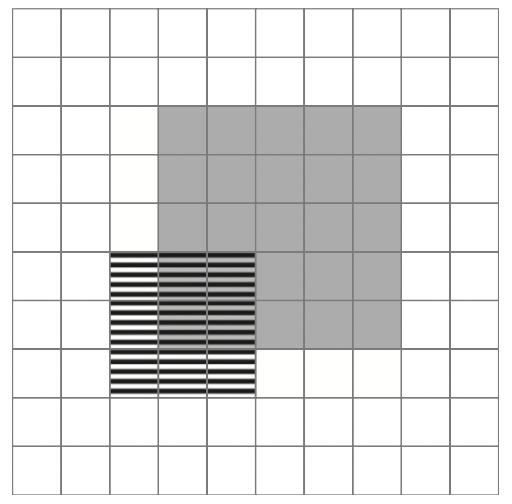
\includegraphics[scale=0.45]{slika1.png}
    \caption{Populacija, predstavljena s 100 kvadrati, z 9 črtastimi, 25 sivimi in 4 črtastimi in sivimi}\vspace{2mm}
 \end{figure}
Slika 2 prikazuje izjeme pri tožilčevi zmoti, predstavljeni na sliki 1. Sedaj imamo 16 črtastih kvadratov, 16 sivih in 4 pikčaste in sive kvadrate, ker je splošna 
razširjenost črtastih in sivih kvadratov enaka, je
\[ 
    P(\text{črtasto} \lvert \text{sivo}) = P(\text{sivo} \lvert \text{črtasto}).
\]
Tudi 
\[
    P(\text{črtasto} \lvert \text{pikčasto}) = P(\text{pikčasto} \lvert \text{črtasto}),
\]
saj sta obe verjetnosti enaki $0$. Oboje(podobno velike populacija in populacije brez prekrivanja) je ozka izjema zmote. \\
Po drugi strani pa so črtkani kvadrati na sliki 2 v celoti zajeti v sivih kvadratih; tako je 
\[
    P(\text{sivo} \lvert \text{črtkano}) = 1, \quad \text{medtem ko je} \quad P(\text{črtkano} \lvert \text{sivo}) = 0,25. 
\]
Tožilčeva zmota velja, kadar je ena skupina podmnožica druge.

\begin{figure}[!ht]\label{fig:slika2}
    \centering
    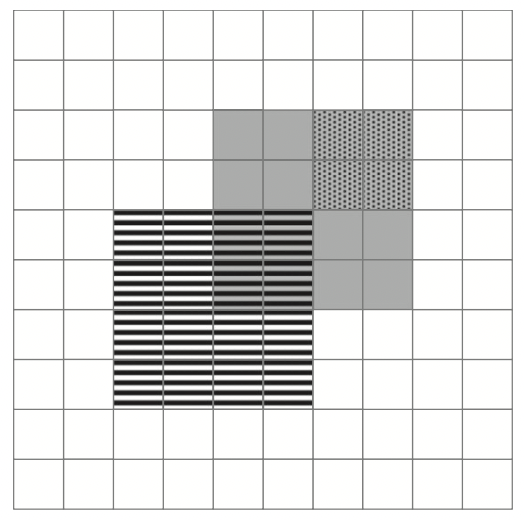
\includegraphics[scale=0.45]{slika2.png}
    \caption{Populacija, predstavljena s 100 kvadrati, z 16 črtastimi, 16 sivimi in 4 pikčastimi in sivimi}\vspace{2mm}
\end{figure}
 

%%%%%%%%%%%%%%%%%%%%%%%%%%%%%%%%%%%%%%%%%%%%%%%%%%%%%%%%%%%%%%%%%%%%%%%%%%%%%%%%%%%%%%%%%%%%%%%%%%%%%%%%%%%%%%%%%%%%%%%%%%%%%%%%%%%%%%%%%%%%%%
%%%%%%%%%%%%%%%%%%%%%%%%%%%%%%%%%%%%%%%%%%%%%%%%%%%%%%%%%%%%%%%%%%%%%%%%%%%%%%%%%%%%%%%%%%%%%%%%%%%%%%%%%%%%%%%%%%%%%%%%%%%%%%%%%%%%%%%%%%%%%%
\section{Izogibanje zmotam z uporabo razmerja verjetnosti}
Vsem zgoraj opisanim zmotam je skupno to, da je resnična koristnost dokaza predstavljena na zavajajoč način - bodisi je pretirana bodisi podcenjena. 
Prednost uporabe razmerja verjetnosti je, da odpravlja ugovorov Bayesovemu izreku, in sicer obveznost upoštevanja predhodne verjetnosti za hipotezo, 
kot je "kriv" (tj. kot sta A ali B na sliki 3, nam ni treba upoštevati predhodne verjetnosti). V veliki meri pomiri pomisleke pravnikov, 
ki bi sicer zavrnili Bayesov argument z utemeljitvijo, da je nedopustno predpostavljati predhodne verjetnosti o krivdi ali nedolžnosti.\\\\
Čeprav je uporaba razmerja verjetnosti kot sredstva za izogibanje zmotam in merjenje uporabnosti dokazov močno podprta, sem vseeno mnenja, da 
imajo, po prebiranju različnih sodb, pravniki in laiki pogosto podobne težave pri razumevanju razmerja verjetnosti kot pri razumevanju 
Bayesove teorije. 

%%%%%%%%%%%%%%%%%%%%%%%%%%%%%%%%%%%%%%%%%%%%%%%%%%%%%%%%%%%%%%%%%%%%%%%%%%%%%%%%%%%%%%%%%%%%%%%%%%%%%%%%%%%%%%%%%%%%%%%%%%%%%%%%%%%%%%%%%%%%%%
%%%%%%%%%%%%%%%%%%%%%%%%%%%%%%%%%%%%%%%%%%%%%%%%%%%%%%%%%%%%%%%%%%%%%%%%%%%%%%%%%%%%%%%%%%%%%%%%%%%%%%%%%%%%%%%%%%%%%%%%%%%%%%%%%%%%%%%%%%%%%%


\end{document}